\let\negmedspace\undefined
\let\negthickspace\undefined
\documentclass[journal]{IEEEtran}
\usepackage[a5paper, margin=10mm, onecolumn]{geometry}
%\usepackage{lmodern} % Ensure lmodern is loaded for pdflatex
\usepackage{tfrupee} % Include tfrupee package

\setlength{\headheight}{1cm} % Set the height of the header box
\setlength{\headsep}{0mm}  % Set the distance between the header box and the top of the text

\usepackage{gvv-book}
\usepackage{gvv}
\usepackage{cite}
\usepackage{amsmath,amssymb,amsfonts,amsthm}
\usepackage{algorithmic}
\usepackage{graphicx}
\usepackage{textcomp}
\usepackage{xcolor}
\usepackage{txfonts}
\usepackage{listings}
\usepackage{enumitem}
\usepackage{mathtools}
\usepackage{gensymb}
\usepackage{comment}
\usepackage[breaklinks=true]{hyperref}
\usepackage{tkz-euclide} 
\usepackage{listings}
% \usepackage{gvv}                                        
\def\inputGnumericTable{}                                 
\usepackage[latin1]{inputenc}                                
\usepackage{color}                                            
\usepackage{array}                                            
\usepackage{longtable}                                       
\usepackage{calc}                                             
\usepackage{multirow}                                         
\usepackage{hhline}                                           
\usepackage{ifthen}                                           
\usepackage{lscape}
\begin{document}

\bibliographystyle{IEEEtran}
\vspace{3cm}

\title{10.4.2.3}
\author{EE24BTECH11021 - Eshan Ray}

% \maketitle
% \newpage
% \bigskip
{\let\newpage\relax\maketitle}

\renewcommand{\thefigure}{\theenumi}
\renewcommand{\thetable}{\theenumi}
\setlength{\intextsep}{10pt} % Space between text and floats

\textbf{Question:}\\
Find two numbers whose sum is $27$ and product is $182$\\
\solution{
Let one of the numbers be $x$\\
So, the other number is $27-x$\\
Given,
\begin{align}
    x\brak{27-x} &= 182\\
    27x-x^2 &=182\\
    x^2 - 27x + 182 &=0\\
    \brak{x-13}\brak{x-14} &= 0\\
    \implies    x &= 13,14
\end{align}

So, the numbers are $13$ and $14$\\

\textbf{Computational Solution:}\\
Using Newton- Raphson Method we get,\\ \\
We start by taking an initial guess and then iteratively we us the following equation to find the roots of the quadratic equation :-
\begin{align}
    x_{n+1} &= x_n - \frac{f\brak{x_n}}{f\prime\brak{x_n}}\\
    f\brak{x} &= x^2 - 27x +182\\
    f\prime\brak{x} &= 2x - 27\\
    x_{n+1} &= x_n - \frac{x_{n}^2-27x_n+182}{2x_n-27}
\end{align}
After running the code, we obtained the following results:-
\begin{align}
    \text{Root-1:}\, 14.00000000\\
    \text{Root-2:}\, 13.00000000
\end{align}

\begin{figure}[H]
    \centering
    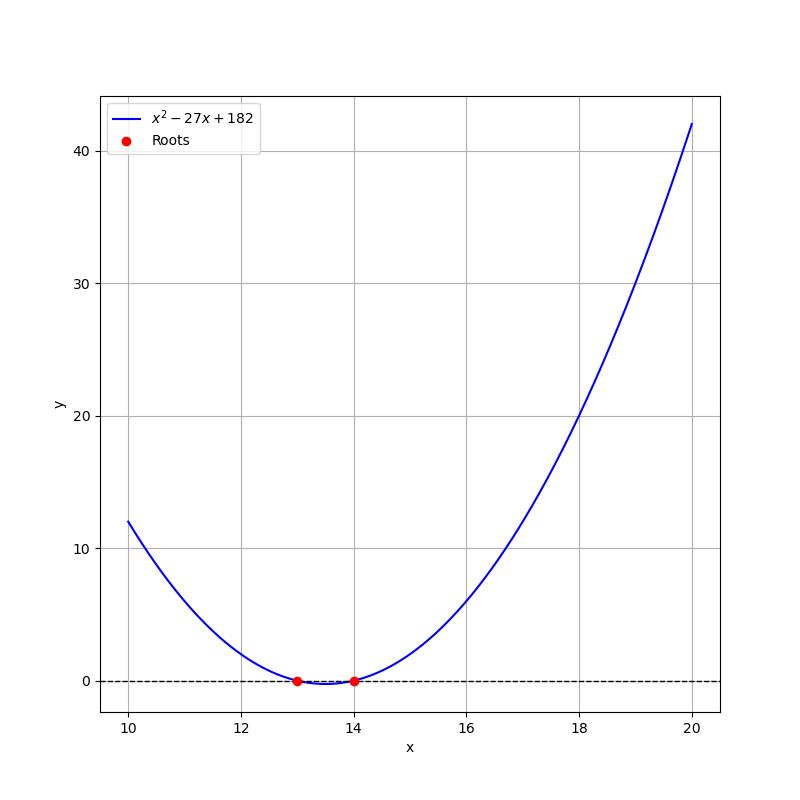
\includegraphics[width=\columnwidth]{plots/plot1.png}
    \caption{Plot of the quadratic equation using newton-Raphson method}
    \label{fig:Plot1}
    \end{figure}

\textbf{Alternate Method: Eigenvalues of Companion Matrix}\\
In this method, we find the roots of any polynomial of the form $x^n + a_{n-1}x^{n-1}\dots ax+a_0=0$ by finding the eigenvalues of the Companion Matrix $\brak{C}$ given below:-\\
\begin{align}
    C &= \myvec{0&1&0&\dots&0\\ 0&0&1&\dots&0\\ \vdots &\vdots &\vdots &\ddots&\vdots\\0&0&0&\vdots&1\\-a_0&-a_1&-a_2&\dots&-a_{n-1}}
\end{align}
For the Quadratic Equation $x^2-27x+182-0$, we get the following companion Matrix
\begin{align}
    C&=\myvec{0&1\\-182&27}
\end{align}
The roots of the equation is the eigenvalues of the matrix $C$ which has been calculated using the QR Decomposition with shifts process.\\
The details of the process is given below:-\\

\textbf{QR Decomposition : Gram-schmidt Process}
\begin{enumerate}
    \item  In the QR Decomposition, the matrix $A$ is decomposed into matrices $Q$ and $R$ as:
    \begin{align}
    A&=QR
    \end{align}
    where ,$Q$ is an orthogonal matrix and $R$ is an upper triangular matrix.
    \item We start by producing an orthogonal set of column vectors of $Q$ \( \{ q_1, q_2, \dots, q_n \} \) from a set of column vectors of $A$ \( \{ a_1, a_2, \dots, a_n \} \).
    \item For orthogonalization we subtract each vector $a_i$ with the projections of all previously obtained orthogonal vectors $q_1,q_2,\dots,q_{i-1}$ to make $q_i$ orthogonal to them. \\
    The projection of $a_i$ onto a vector $q_j$ is calculated as:
    \begin{align}
    proj_{q_j}(a_i) &= \frac{\langle a_i,q_j\rangle}{\langle q_j,q_j\rangle}q_j
    \end{align}
    Then $q_i$ is computed as:
    \begin{align}
    q_i &= a_i- \sum_{j=1}^{i-1}proj_{q_j}(a_i)
    \end{align}
    Then all the $q_i$'s are normalized by :
    \begin{align}
    q_i &= \frac{q_i}{||q_i||}
    \end{align}
    The process is repeated for all the colums of $A$
    \item[3)] As $Q$ is an orthonormal matrix
    \begin{align}
        Q^\top Q &=I
    \end{align}
    So, $R$ can be represented as follows
    \begin{align}
        R &= Q^\top A\\
        r_{ij} &= \langle a_j, q_i \rangle \text{ , for  }  i \leq j 
    \end{align}
\end{enumerate}
    \textbf{ QR algorithm:}\\
    In the  QR algorithm, the matrix $A_n$ is decomposed into matrices $Q_n$ and $R_n$ as:
    \begin{align}
    A_{n}&=Q_nR_n
    \end{align}
Then, the new matrix $A_{n+1}$ is computed as:
\begin{align}
A_{n+1}&=R_nQ_n
\end{align}
This process is repeated until the off-diagonal elements of the matrix become negligibly small, at which point the diagonal elements approximate the eigenvalues of the original matrix.\\ \\
 \begin{align}
	\text{Eigenvalues computed :}\, [14.0, 13.0]
\end{align}
\begin{figure}[h]
    \centering
    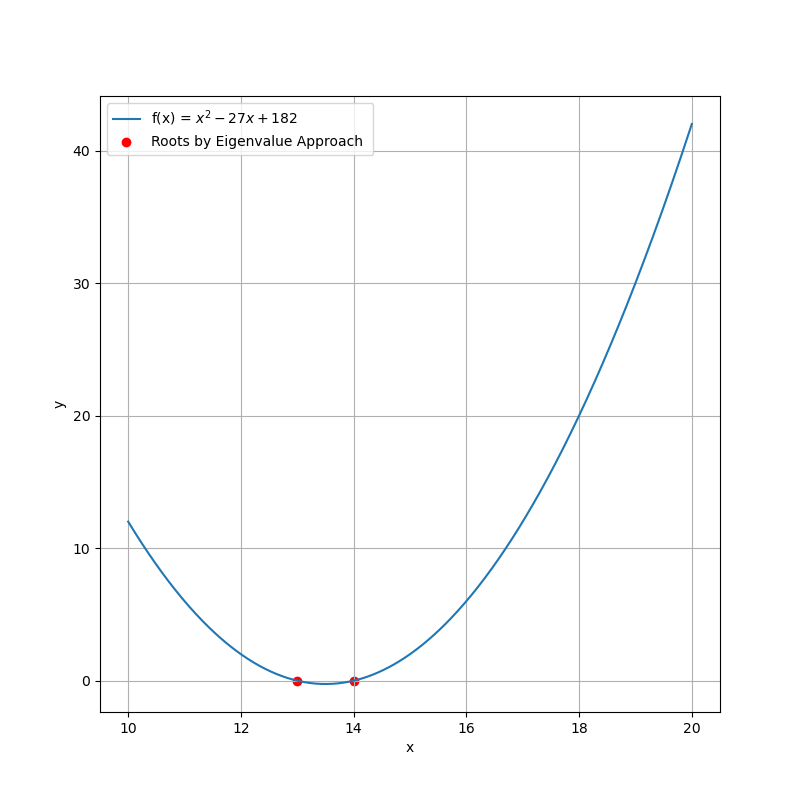
\includegraphics[width=\columnwidth]{plots/plot2.png}
    \caption{Plot of the quadratic equation by eigenvalue approach}
    \label{fig:Plot1}
    \end{figure}
}
\end{document}



